\chapter {Utilisation basique de Buildroot}
\begin{centering}
  
\includegraphics[height=0.1\textheight]{pictures/br.png} \\
\end{centering}
{Objectifs:
  \begin{itemize}
  \item Télécharger Buildroot
  \item Configurer un système minimal avec Buildroot pour la Raspberry Pi 3
  \item Lancer la compilation
  \item Flasher et tester le système généré
  \end{itemize}
}

%%%%%%%%%%%%%%%%%%%%%%%%%%%%%%%
\section{Setup}
%%%%%%%%%%%%%%%%%%%%%%%%%%%%%%%

Comme spécifié dans la documentation Buildroot\footnote{\url{https://buildroot.org/downloads/manual/manual.html\#requirement-mandatory}}, vous avez besoin de certains paquets/dépendances :

\begin{verbatim}
sudo apt install sed make binutils gcc g++ bash patch \
  gzip bzip2 perl tar cpio python unzip rsync wget libncurses-dev
\end{verbatim}

Lisez les spécificités de votre carte RPi3 sur différents sites notamment \href{https://www.raspberrypi.org/products/raspberry-pi-3-model-b/}{le site de la Raspberry Fondation}

%%%%%%%%%%%%%%%%%%%%%%%%%%%%%%%
\section{Télécharger Buildroot}
%%%%%%%%%%%%%%%%%%%%%%%%%%%%%%%

Comme nous allons réaliser du développement Buildroot, on va télécharger les sources depuis le répertoire Git :

\begin{verbatim}
git clone git://git.busybox.net/buildroot
\end{verbatim}

Aller dans le nouveau dossier \code{buildroot} créé.

Nous allons utiliser la branche {\em 2019.08} de cette release.

\begin{verbatim}
git checkout 2019.08
\end{verbatim}

%%%%%%%%%%%%%%%%%%%%%%%%%%%%%%%
\section{Configuration de Buildroot}
%%%%%%%%%%%%%%%%%%%%%%%%%%%%%%%

Si vous regardez le dossier \code{configs/}, vous verrez qu'il y a un fichier
\code{raspberrypi3_defconfig}, qui est une configuration pour construire
un système pour une Raspberry Pi 3. Faites donc un:

\begin{verbatim}
make raspberrypi3_defconfig
\end{verbatim}

Mais comme on souhaite apprendre Buildroot, on va regarder la configuration
un peu plus en détails.

Démarrez l'utilitaire de configuration Buildroot :

\begin{verbatim}
make menuconfig
\end{verbatim}

Il est aussi possible d'utiliser les autres outils comme \code{nconfig},
\code{xconfig} ou \code{gconfig}.

Maintenant, regardons les points importants Buildroot:
\begin{itemize}
\item Menu \code{Target Options}
  \begin{itemize}
  \item \code{Target Architecture} : \code{ARM (little endian)}
  \item \code{Target Architecture Variant} : D'après le
    \href{https://www.raspberrypi.org/products/raspberry-pi-3-model-b/}{site web de la RPi3},
    ils utilisent un CPU Broadcom BCM2837 qui est basé sur ARM \code{Cortex-A53}
  \end{itemize}
\item Menu \code{Build options} : Regardez notamment le lieu où sauver la
  configuration Buildroot
\item Menu \code{Toolchain}
  \begin{itemize}
  \item Par défaut, Buildroot compile sa propre toolchain. Ca prend un peu
    de temps même si pour \code{ARMv8} il y a une toolchain pré-buildée fournie par
    ARM.% Selectionnez \code{External toolchain} comme \code{Toolchain type}.
%  \item Selectionnez \code{Arm ARM 2019.03} comme \code{Toolchain}.
  \end{itemize}
\item Menu \code{Kernel}
  \begin{itemize}
  \item Par défaut, le kernel le plus récent dans la release Buildroot est
    utilisé. Ici, il s'agit d'un kernel spécifique, sur github d'où le
    \code{Custom Tarballs}
  \item Faites attention à la configuration kernel utilisé
    \code{Using an in-tree defconfig file} avec \code{bcm2709} comme
    configuration. Correspond au ficher \code{bcm2709_defconfig} dans le
    kernel: \url{https://github.com/raspberrypi/linux/blob/rpi-4.19.y/arch/arm/configs/bcm2709_defconfig}
  \item Sur ARM, beaucoup de plateformes utilisent un {\em Device Tree} pour
    décrire le hardware. Vous pouvez regarder son DT :
    \url{https://github.com/raspberrypi/linux/blob/rpi-4.19.y/arch/arm/boot/dts/bcm2710-rpi-3-b.dts},
  \end{itemize}

\item Menu \code{Target packages}. Surement le plus important
  car c'est le menu qui permet d'installer les paquets souhaités dans
  le rootfs final. On verra dans un autre lab un exemple.
\item Menu \code{Filesystem images}. Pour savoir quel type d'image on veut
  générer.
\item Menu \code{Bootloaders}
  \begin{itemize}
  \item Le plus populaire pour ARM est {\em U-Boot}. Pour la RPi3 n'a pas
    besoin d'un bootloader pour executer et charger le kernel donc pas besoin!
  \end{itemize}

\end{itemize}

%%%%%%%%%%%%%%%%%%%%%%%%%%%%%%%
\section{Compilation}
%%%%%%%%%%%%%%%%%%%%%%%%%%%%%%%

Simplement lancez \code{make} ou redirigez la sortie avec la commande
\code{tee}:

\begin{verbatim}
make 2>&1 | tee build.log
\end{verbatim}

%%%%%%%%%%%%%%%%%%%%%%%%%%%%%%%
\section{Flasher la carte SD}
%%%%%%%%%%%%%%%%%%%%%%%%%%%%%%%

Une fois la compilation terminée, on va pouvoir flasher notre système
sur notre carte SD. Mais avant, encore faut-il l'identifier !
Regardez la sortie de \code{cat /proc/partitions} et
chercher votre carte SD. En géneral, un lecteur de carte SD donnera
\code{mmcblk0}, alors qu'un lecteur externe USB, ça sera du type
\code{sdX} (i.e\code{sdb}, \code{sdc}, etc.). {\bf Attention :
  \code{/dev/sda} est généralement le disque dur de votre laptop!}

Si votre carte SD est \code{/dev/mmcblk0}, les partitions seront
\code{/dev/mmcblk0p1}, \code{/dev/mmcblk0p2}, etc. Si c'est \code{/dev/sdc},
les partitions seront \code{/dev/sdc1}, \code{/dev/sdc2}, etc.

Pour flasher votre système, suivez la commande indiquée dans le \code{README}
de la RPi3 : \url{https://git.buildroot.net/buildroot/tree/board/raspberrypi/readme.txt?h=2019.08}: \\

\begin{verbatim}
sudo dd if=output/images/sdcard.img of=/dev/mmcblk0 bs=1M
\end{verbatim}

Ou \code{sdc} ou \code{sdb} au lieu de \code{mmcblk0} si besoin.

%%%%%%%%%%%%%%%%%%%%%%%%%%%%%%%
\section{Démarrage du système}
%%%%%%%%%%%%%%%%%%%%%%%%%%%%%%%

Insérez la carte SD dans la RPi3.\\
Branchez la série selon les pins de votre RPi3 :

\begin{centering}
  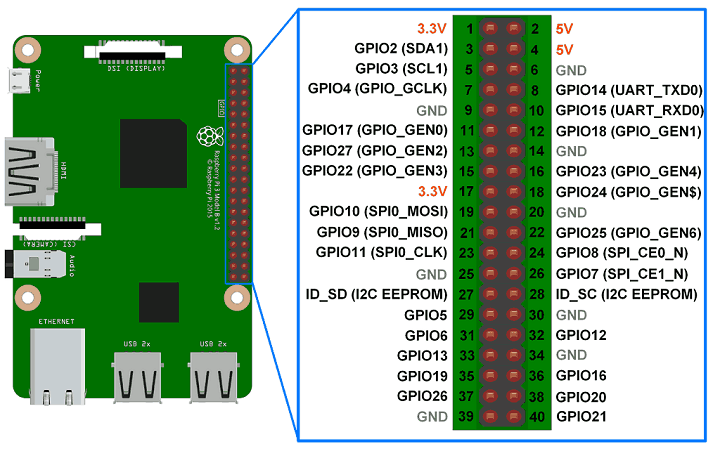
\includegraphics[height=0.5\textheight]{pictures/04_labs/rpi3_gpio_layout.png} \\
\end{centering}

Allumez via USB votre board et vous devriez voir le système booter !

Le login est \code{root} et profitez pour explorer le système. Lancer
\code{ps} pour regarder combien de processus sont en cours d'exécution,
qu'est-ce que Buildroot a généré dans \code{/bin}, \code{/lib}, \code{/usr}
et \code{/etc}.

%%%%%%%%%%%%%%%%%%%%%%%%%%%%%%%
\section{Explorer le log de build}
%%%%%%%%%%%%%%%%%%%%%%%%%%%%%%%

De retour sur votre machine de build, regardez la sortie du log \code{build.log}.
Buildroot est un peu verbose mais il affichera chaque message important d'un
prefixe \code{>>>}. Pour avoir une idée générale de ce qui a été fait, vous
pouvez lancer:

\begin{verbatim}
grep ">>>" build.log
\end{verbatim}

Vous voyez les différents paquets être téléchargés, extraits, patchés,
configurés compilés et installés.
